%%%%%%%%%%%%%%%%%%%%%%%%%%%%%%%%%%%%%%%%%
% Simple Sectioned Essay Template
% LaTeX Template
%
% This template has been downloaded from:
% http://www.latextemplates.com
%
% Note:
% The \lipsum[#] commands throughout this template generate dummy text
% to fill the template out. These commands should all be removed when 
% writing essay content.
%
%%%%%%%%%%%%%%%%%%%%%%%%%%%%%%%%%%%%%%%%%

%----------------------------------------------------------------------------------------
%	PACKAGES AND OTHER DOCUMENT CONFIGURATIONS
%----------------------------------------------------------------------------------------

\documentclass[12pt]{article} % Default font size is 12pt, it can be changed here

\usepackage{geometry} % Required to change the page size to A4
\geometry{a4paper} % Set the page size to be A4 as opposed to the default US Letter

\usepackage{graphicx} % Required for including pictures

\usepackage{float} % Allows putting an [H] in \begin{figure} to specify the exact location of the figure
\usepackage{wrapfig} % Allows in-line images such as the example fish picture

\usepackage{lipsum} % Used for inserting dummy 'Lorem ipsum' text into the template

\usepackage{url}

\linespread{1.2} % Line spacing

%\setlength\parindent{0pt} % Uncomment to remove all indentation from paragraphs

\newcommand{\figref}[1]{Figure~\ref{#1}}
\graphicspath{{./figures/}} % Specifies the directory where pictures are stored

\begin{document}

%----------------------------------------------------------------------------------------
%	TITLE PAGE
%----------------------------------------------------------------------------------------

\begin{titlepage}

\newcommand{\HRule}{\rule{\linewidth}{0.5mm}} % Defines a new command for the horizontal lines, change thickness here

\center % Center everything on the page

\HRule \\[0.4cm]
{ \huge \bfseries Alpha Data ADM-PCIE-7v3 Memory Bandwidth Test}\\[0.4cm] % Title of your document
\HRule \\[1.5cm]

\begin{minipage}{0.4\textwidth}
    \centering {Cheng Liu} \\ 
    \vspace{2em}
    \centering {\large \today}
\end{minipage}

\end{titlepage}

%----------------------------------------------------------------------------------------
%	TABLE OF CONTENTS
%----------------------------------------------------------------------------------------

%\tableofcontents % Include a table of contents

%\newpage % Begins the essay on a new page instead of on the same page as the table of contents 

%----------------------------------------------------------------------------------------
%	INTRODUCTION
%----------------------------------------------------------------------------------------
\section{Memory Bandwidth Test Report} % Major section
In order to get an overview of the memory bandwidth of the ADM-PCIE-7v3 board, 
we have both sequential and random memory access bandwidth tested. Half of the memory access 
is read and the other half is write. Also note that 
there are two different pieces of memory on the system. The host DDR memory and the 
FPGA DDR memory. Here we just tested the bandwidth of the FPGA DDR memory bandwidth 
accessed from FPGA. As it is the probably the bottleneck for memory intensive 
applications running on FPGA.

Figure \figref{fig:seq-access} and Figure \figref{fig:rnd-access} show the measured memory 
bandwidth with sequential memory access and random access respectively. Basically, it can be 
found that sequential memory access bandwidth drops dramatically when the data size gets smaller 
while the random memory access is relatively less senseitive to the data size. Meanwhile, the sequential 
memory access is a dozens of times more efficient than the random memory access.

Another thing is that the Alpha-Data ADM-PCIE-7v3 board has two SODIMM DDR. Each of them can goes up to 
1333MT/s i.e. 10.6GB/s according to the spec \cite{adm-pcie-7v3}. However, we can only utilize one 
SODIMM on the FPGA due to the DSA provided in SDAccel and the best bandwidth that we can achieve in 
sequential access manner is around 8.6GB/s.

\begin{figure}[htb]
	\centering
	\label{fig:seq-access}
	\caption{Memory Bandwidth with Sequential Memory Access}
	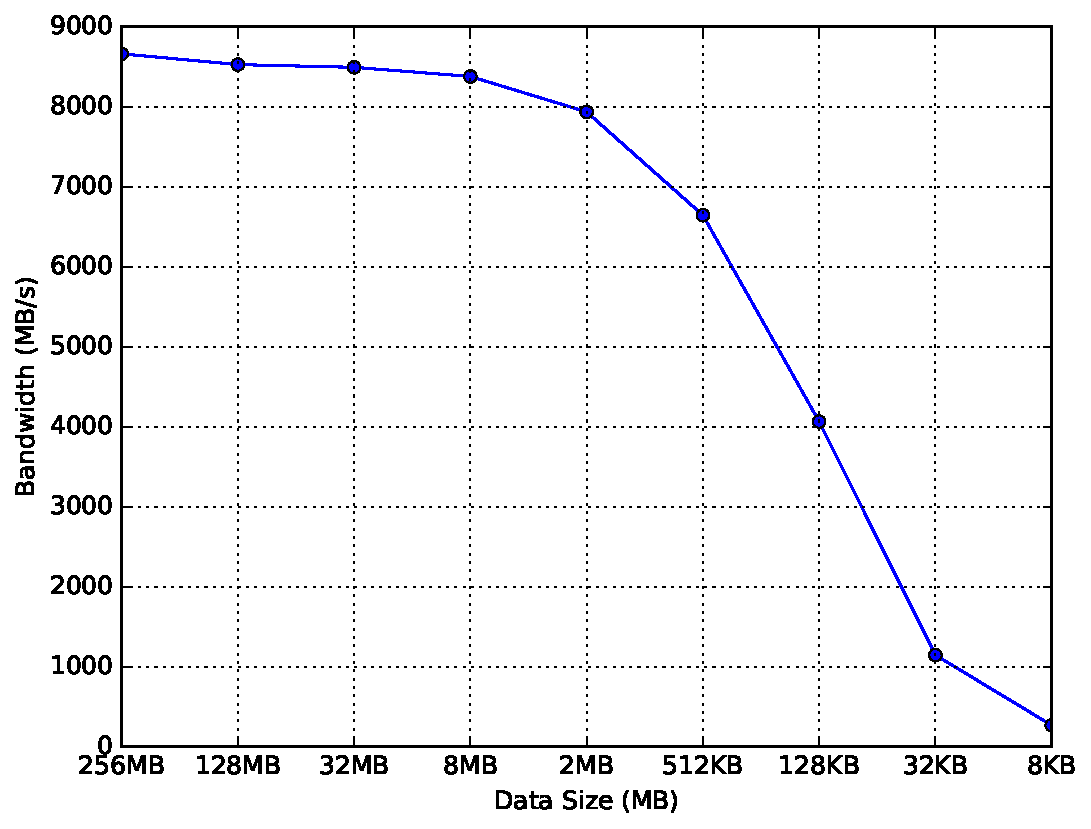
\includegraphics[width=.7\linewidth]{seq_access}
\end{figure}

\begin{figure}[htb]
	\centering
	\label{fig:rnd-access}
	\caption{Memory Bandwidth with Random Memory Access}
	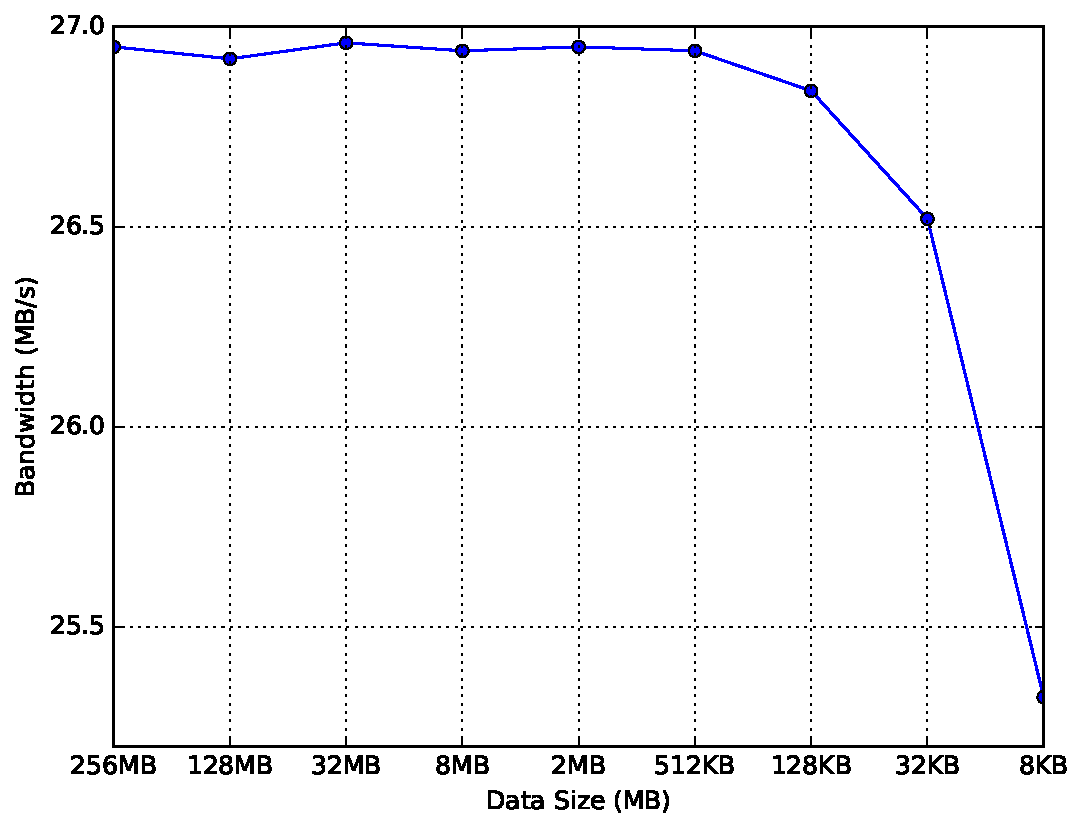
\includegraphics[width=.7\linewidth]{rnd_access}
\end{figure}




%----------------------------------------------------------------------------------------
%	BIBLIOGRAPHY
%----------------------------------------------------------------------------------------
\bibliographystyle{plain}
\bibliography{refs}
%----------------------------------------------------------------------------------------

\end{document}
